\section{Own Experiments}
\label{own-experiments}


\end{multicols}

\begin{figure}
    \centering
    \begin{subfigure}[b]{0.4\textwidth}
        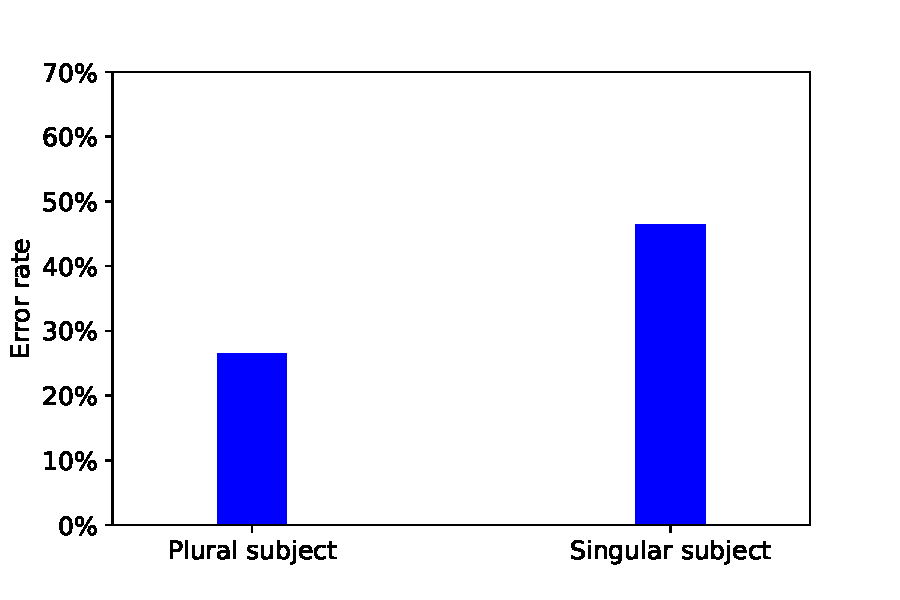
\includegraphics[width=\textwidth]{2b_least.pdf}
        \label{fig:2b}
    \end{subfigure}
    ~ %add desired spacing between images, e. g. ~, \quad, \qquad, \hfill etc. 
      %(or a blank line to force the subfigure onto a new line)
              \caption{Error rates of the language model plotted against: 2a presence and number of last intervening noun; 1b count of attractors in dependencies with homogeneous intervention}
\end{figure}
\begin{multicols}{2}


To predict the correct number of a given verb,
the language model should be able to
1. identify the noun that is the head of the subject for the verb
2. establish the number of the noun (non-trivial since no knowledge of -s postfix for plurals)
3. establish the number of the given verb forms (also non-trivial).

In the first sub section we investigate if our model is able to
do this for simple cases with only a single noun in the prefix.
%
In the second sub section we investigate if our model can handle
more complex cases with two nouns in the prefix,
and what information it then uses to identify the head of the subject.

\subsection{Noun-Verb Agreement in Simple Cases}


In this section we investigate the ability of the model to
establish number agreement for nouns and verbs in the simplest case,
following the pattern: ``The <noun> <verb>''. Notice that
the determiner ``The'' clearly indicates the position of the noun.

1. TEST DATA: 
Generate 1000 simple prefixes in singular and plural form, like ``the company ... [produce/produces]'' 
and ``the companies ... [produce/produces]''.
The sentences do not need to be meaningful.
(randomly pick the nouns and verbs without taking into account their frequency in training data)

2. EXPERIMENT: 
Evaluate how the language model performs on these sentences 
and conclude whether or not the model is sensitive to noun-verb agreement in simple cases. 
(i.e. if it tends to predict plural verbs for plural nouns and singular verbs for singular nouns)
output 1: cross table with correct vs predicted
output 2: overall error rate number, error rate number for plurals, error rate number for singulars 


2. FURTHER ANALYSIS:
hypothesis: the model falls back to pure frequencies of the two verb forms
in case it failed to learn the counts because of sparsity in the data.

Further inspect the error cases, why did it fail for these very simple sentences:
a) maybe the model failed to learn the number of the noun (i.e. low occurrence in training data for the given noun form)?
b) maybe the model failed to learn the number of the verb forms (i.e. low occurrence in training data for both verb forms)?
c) maybe the occurence in the training data of the incorrect but predicted verb form is much higher than the occurrence 
in training data of the correct form?
%output a: histogram with x-axis z-score noun, y axis count (or percentage) of verbs that fall in this range
%output b: histogram with x-axis z-score verb (max of both), y axis count (or percentage) of verbs that fall in this range
%output c: histogram with x-axis percentage of predicted form, y axis count (or percentage) of verbs that fall in this range
output(?): a scatter plot, x-axis z-score noun vs y-axis z-score verb, color gradient is percentage of predicted verb form

\subsubsection{Distance}

(maybe we can just refer to the replication section)

The ability of the model to track the number of a noun may degrade
when the noun and the verb are far apart.
Below we investigate the effect of distance on number agreement for simple,
single noun, cases.

1. TEST DATA:
Pick the simple cases and generate multiple additional cases for each by adding 0 to n additional words (randomly picked from a set of non-nouns)
[preferable: use real sentences of different length without attractors for this]

2. EXPERIMENT:
Evaluate how the language model performs on these sentences 
and conclude whether or not the model is robust to distance. 
(i.e. if it tends to predict plural verb for plural nouns even when they are far apart)
output: line diagram with x-axis distance (number of words inbetween), y-axis error rate
 
\subsection{Noun-Verb Agreement in Complex Cases}

When multiple nouns in the prefix, how does the model 'pick' the noun to agree with?
Most recent noun is a simple heuristic, but maybe it can do better based
on the available information?

\subsubsection{Syntactic Information}

We first look at syntactic clues such as punctuation
and function words such as 'that' or 'of'
that indicate the start of a relative resp. possesive
clause. Do these words help the model to pick
the noun that serves as the head of the sentence?

1. TEST DATA:
Generate sentences using different templates, singular and plural formats:
"The [Noun1] of the [Noun2] ..."
"The [Noun1] and the [Noun2] ..."
"The [Noun1] that the [Noun2] ..."
"The [Noun1] , that the [Noun2] ..."
"The [Noun1] the [Noun2] ..."
...
Discuss templates and function words.
[Remark: pick noun/verb combinations for which the simple cases succeed?!]

2. EXPERIMENT:
Evaluate how much the language model tends to agree with the last noun 
(correct for some templates, erroneous for others)
output: bar chart with template-id on x axis, percentage of agreement
with last noun on y axis, color green if correct, color red if erroneous.  

3. ANALYSIS:
The model is less likely to agree with the number of the 
last noun in case it has syntactic information
that points in the direction of the first noun as the head of the subject.
(green bars are significantly higher than red bars,
templates with relativizer scores better than without)
Is this indeed the case ???

\subsubsection{Semantic Information}

We now look at semantic clues, i.e. companies
are more likely to produce than employees.

1. TEST DATA:
Find VBP-NNS (resp. VBZ-NN) pairs so that VBP and NNS (resp. VBZ and NN) frequently occur together in a sentence (example: prices stabilize).
Now generate prefixes using an attractor template, for example: "The NNS of the [NN] ...[VBZ/VBP]",
with NN randomly picked and VBZ created by adding an 's' (and checking if this format exists as VBZ). 
Remark: 'frequently occur together' means: count(VBP + NNS)/count(VBP) is high.
Remark: for proper comparison it makes sense to also create "The NNS* of the [NN] ...[VBZ/VBP]"
with NNS* randomly picked as a baseline set.
For example, we add "The prices of the employee ... [stabilize/stabilizes]" to our testset
and "The companies of the employee ... [stabilize/stabilizes]" to our comparison test.

EXPERIMENT:
Evaluate our model on the constructed testset and on the comparison set.
If the model scores significantly better on the testset
then it shows sensitivity to semantic clues.

(remark: we can repeat the experiment with the nouns interchanged and check that we score worse now,
e.g. "The employee that the prices ... [stabilize/stabilizes]" 
In that case syntax and semantics are inconsistent)